%%%%%%%%%%%%%%%%%%%%%%%%%%%%%%%%%%%%%%%%%%%%%%%%%%%%%%%%%%%%%%%%%
%  _____   ____  _____                                          %
% |_   _| /  __||  __ \    Institute of Computitional Physics   %
%   | |  |  /   | |__) |   Zuercher Hochschule Winterthur       %
%   | |  | (    |  ___/    (University of Applied Sciences)     %
%  _| |_ |  \__ | |        8401 Winterthur, Switzerland         %
% |_____| \____||_|                                             %
%%%%%%%%%%%%%%%%%%%%%%%%%%%%%%%%%%%%%%%%%%%%%%%%%%%%%%%%%%%%%%%%%
%
% Project     : Pflichtenheft für WeKeBA
% Title       : 
% File        : doc.tex Rev. 00
% Date        : 15.09.2014
% Author      : Tobias Welti
%
%%%%%%%%%%%%%%%%%%%%%%%%%%%%%%%%%%%%%%%%%%%%%%%%%%%%%%%%%%%%%%%%%

%%%%%%%%%%%%%%%%%%%%%%%%%%%%%%%%%%%%%%%%%%%%%%%%%%%%%%%%%%%%%%%%%
%  _____   ____  _____                                          %
% |_   _| /  __||  __ \    Institute of Computitional Physics   %
%   | |  |  /   | |__) |   Zuercher Hochschule Winterthur       %
%   | |  | (    |  ___/    (University of Applied Sciences)     %
%  _| |_ |  \__ | |        8401 Winterthur, Switzerland         %
% |_____| \____||_|                                             %
%%%%%%%%%%%%%%%%%%%%%%%%%%%%%%%%%%%%%%%%%%%%%%%%%%%%%%%%%%%%%%%%%
%
% Project     : Konzept BA Welti Keller
% Title       : 
% File        : header.tex Rev. 00
% Date        : 15.09.2014
% Author      : Tobias Welti
%
%%%%%%%%%%%%%%%%%%%%%%%%%%%%%%%%%%%%%%%%%%%%%%%%%%%%%%%%%%%%%%%%%

\documentclass[twoside,10pt,parskip=half,ngerman]{scrreprt}

%***********************************************************************
% include some libs
%***********************************************************************	
\usepackage[utf8]{inputenc}
\usepackage{listings}
\usepackage{color}
\usepackage{fancyhdr}
\usepackage{rotating}
\usepackage{titlesec}
\usepackage{mathptmx}
\usepackage{todonotes}
 \usepackage{helvet}
%\usepackage[scaled]{uarial}
\renewcommand*\familydefault{\sfdefault} %% Only if the base font of the document is to be sans serif
\usepackage[T1]{fontenc}
\usepackage{ngerman}
\usepackage{textcomp}
\usepackage[squaren]{SIunits}
\usepackage{graphicx}
\usepackage[hyphens]{url}
\usepackage{geometry}
\usepackage[absolute]{textpos}
\usepackage{makeidx}
\usepackage{colortbl}
\usepackage{pdflscape}
\usepackage{pdfpages}
\usepackage{tabularx}
\usepackage{lmodern}
\usepackage{longtable}
\usepackage{array}
\usepackage{float}
\usepackage{scrhack}
\usepackage[plainpages=false]{hyperref}
\usepackage{wallpaper}
\usepackage{hyperref}
\urlstyle{same}

% Glossar
\usepackage[toc,nopostdot,acronyms]{glossaries}
%\usepackage{glossaries-german}
\renewcommand*{\glossaryname}{Glossar}
\renewcommand*{\acronymname}{Abkürzungsverzeichnis}
\setacronymstyle{long-short}
\makeglossaries
\loadglsentries{content/glossar}
%\makenoidxglossaries




% Deutsches Literaturverzeichnis
\usepackage{bibgerm}
% Silbentrennung (Neu-Deutsch)
 \usepackage[ngerman]{babel}
 % Spezialseiten (Literarturverzeichnis, Abbildungsverzeichnis, usw.) in Inhaltsverzeichnis anzeigen
\usepackage[nottoc]{tocbibind}

% Grafiken
%\usepackage[pdftex]{graphicx}
%\usepackage{epsfig}

%***********************************************************************
% various styles
%***********************************************************************	

%create index
\makeindex

%define pagestyle
\pagestyle{fancy}

%use sans-serif font 
%\renewcommand{\familydefault}{\sfdefault}

%define page margin
\geometry{a4paper, top=30mm, left=30mm, right=30mm, bottom=30mm,headsep=10mm,footskip=10mm}

%textpos parameter
\setlength{\TPHorizModule}{30mm}
\setlength{\TPVertModule}{\TPHorizModule}
\textblockorigin{10mm}{10mm} % start everything near the top-left corner
\setlength{\parindent}{0pt}

%horizontal lines for titlepage 
\newcommand{\HRule}{\rule{\linewidth}{0.5mm}}

%reference to source items inlc source number
\newcommand{\srcref}[1]{\nameref{src:#1} \cite{#1}}

%header / footer 
\renewcommand{\headrulewidth}{0.3pt}
\renewcommand{\footrulewidth}{0.3pt}

\fancyhead[LO,RE]{} %clear headings for contents 
\fancyhead[RO,LE]{\nouppercase{\rightmark}} %right odd pages and left even pages
\fancyhead[LO,RE]{\MakeUppercase{\leftmark}} %left odd pages and right even pages
\fancyfoot[LE,RO]{\thepage} %page numbering
\fancyfoot[C]{} %clear centered page numbering 

%define some colors
\definecolor{gray}{rgb}{0.95,0.95,0.95}
\definecolor{darkgray}{rgb}{0.4,0.4,0.4}
%listing colors
\definecolor{lgray}{RGB}{250,250,250}
\definecolor{lgreen}{RGB}{63,127,95}
\definecolor{lred}{RGB}{127,0,85}
\definecolor{lblue}{RGB}{42,0,255}

%***********************************************************************
% listing
%***********************************************************************

\lstset{		
		basicstyle=\small\ttfamily,
		frame=single,
		numbers=left,	
		numberstyle=\tiny,
		%firstnumber=auto,
		numberblanklines=true,
		captionpos=b,
		extendedchars=true,
		float=ht,
		showtabs=false,
		tabsize=2,
		showspaces=false,
		showstringspaces=false,
		breaklines=true,
		%prebreak=\Righttorque,
		backgroundcolor=\color{lgray},
		keywordstyle=\color{lred}\bfseries, 
		commentstyle=\color{lgreen}\ttfamily,
%		morekeywords={printstr, printhexln},
		stringstyle=\color{lblue},
		xleftmargin=0.5cm,
		xrightmargin=0.5cm
}

\lstloadlanguages{C++}

%\lstdefinelanguage{xc}{
%     keywords={printstr, printhexln, attributes, class, classend, do, empty, endif, endwhile, fail, function, functionend, if, implements, in, inherit, inout, not, of, operations, out, return, set, then, types, while, use},
%     keywordstyle=\color{lred}\bfseries,
%     ndkeywords={},
%     ndkeywordstyle=\color{yellow}\bfseries,
%     identifierstyle=\color{black},
%     sensitive=false,
%     comment=[l]{//},
%     commentstyle=\color{lgreen}\ttfamily,
%     string=[l]{"},
%     stringstyle=\color{lblue}\ttfamily
%  }


\begin{document}
\title{Bachelorarbeit (IT)}
\author{Tobias Keller, Tobias Welti}

% !TeX spellcheck = de_CH
%%%%%%%%%%%%%%%%%%%%%%%%%%%%%%%%%%%%%%%%%%%%%%%%%%%%%%%%%%%%%%%%%
%  _____   ____  _____                                          %
% |_   _| /  __||  __ \    Institute of Computitional Physics   %
%   | |  |  /   | |__) |   Zuercher Hochschule Winterthur       %
%   | |  | (    |  ___/    (University of Applied Sciences)     %
%  _| |_ |  \__ | |        8401 Winterthur, Switzerland         %
% |_____| \____||_|                                             %
%%%%%%%%%%%%%%%%%%%%%%%%%%%%%%%%%%%%%%%%%%%%%%%%%%%%%%%%%%%%%%%%%
%
% Project     : BA Welti Keller
% Title       : 
% File        : titlepage.tex Rev. 00
% Date        : 15.09.2014
% Author      : Tobias Welti
%
%%%%%%%%%%%%%%%%%%%%%%%%%%%%%%%%%%%%%%%%%%%%%%%%%%%%%%%%%%%%%%%%%

\begin{titlepage}

% Logo
\ThisTileWallPaper{\paperwidth}{\paperheight}{images/logos/InES.pdf} % {}images/logos/*.pdf}
% Wählen Sie aus folenden pdf Files: ICP, IDP, IEFE, IMES, IMPE, IMS, INE, InES, InIT, KSR, SoE, ZAMP, ZAV, ZIL, ZPP, ZSN

\begin{minipage}[b]{0.117\textwidth}
\hskip 0.05cm
\end{minipage}
\begin{minipage}[b]{0.91\textwidth}
\begin{tiny}.\end{tiny}\vskip 2.8cm
	{\huge
	
	% Projekt Name
	\textbf{\underline{Bachelorarbeit}}
	
	% Projekt Titel
	Messstation zur Registrierung von Geschiebe-Bewegungen im Fluss
	\vskip 0.5cm}
	
	\begin{minipage}[b]{0.27\textwidth}
	\hrule\vskip 0.5cm
		\textbf{Autoren}\\
		\\
	\end{minipage}
	\begin{minipage}[b]{0.03\textwidth}
	\hskip 0.5cm
	\end{minipage}
	\begin{minipage}[b]{0.7\textwidth}
	\hrule\vskip 0.5cm
		Tobias Keller\\
		Tobias Welti\\
	\end{minipage}
	
	\begin{minipage}[b]{0.27\textwidth}
	\hrule\vskip 0.5cm
		\textbf{Betreuer}\\
		\\
	\end{minipage}
	\begin{minipage}[b]{0.03\textwidth}
	\hskip 0.5cm
	\end{minipage}
	\begin{minipage}[b]{0.7\textwidth}
	\hrule\vskip 0.5cm
		Prof. Hans-Joachim Gelke, Dipl. El. Ing. FH\\
		ZHAW Institute for Embedded Systems\\
	\end{minipage}
	
	\begin{minipage}[b]{0.27\textwidth}
	\hrule\vskip 0.5cm
		\textbf{Partner}\\
		\\
	\end{minipage}
	\begin{minipage}[b]{0.03\textwidth}
	\hskip 0.5cm
	\end{minipage}
	\begin{minipage}[b]{0.7\textwidth}
	\hrule\vskip 0.5cm
	  Carlos Rodrigo Wyss\\
		Eidg. Forschungsanstalt für Wald, Schnee und Landschaft WSL\\
	\end{minipage}
	
	\begin{minipage}[b]{0.27\textwidth}
	\hrule\vskip 0.5cm
		\textbf{Datum}
	\end{minipage}
	\begin{minipage}[b]{0.03\textwidth}
	\hskip 0.5cm
	\end{minipage}
	\begin{minipage}[b]{0.7\textwidth}
	\hrule\vskip 0.5cm
		\today
	\end{minipage}
\end{minipage}
\vskip 0.5cm

\end{titlepage}

%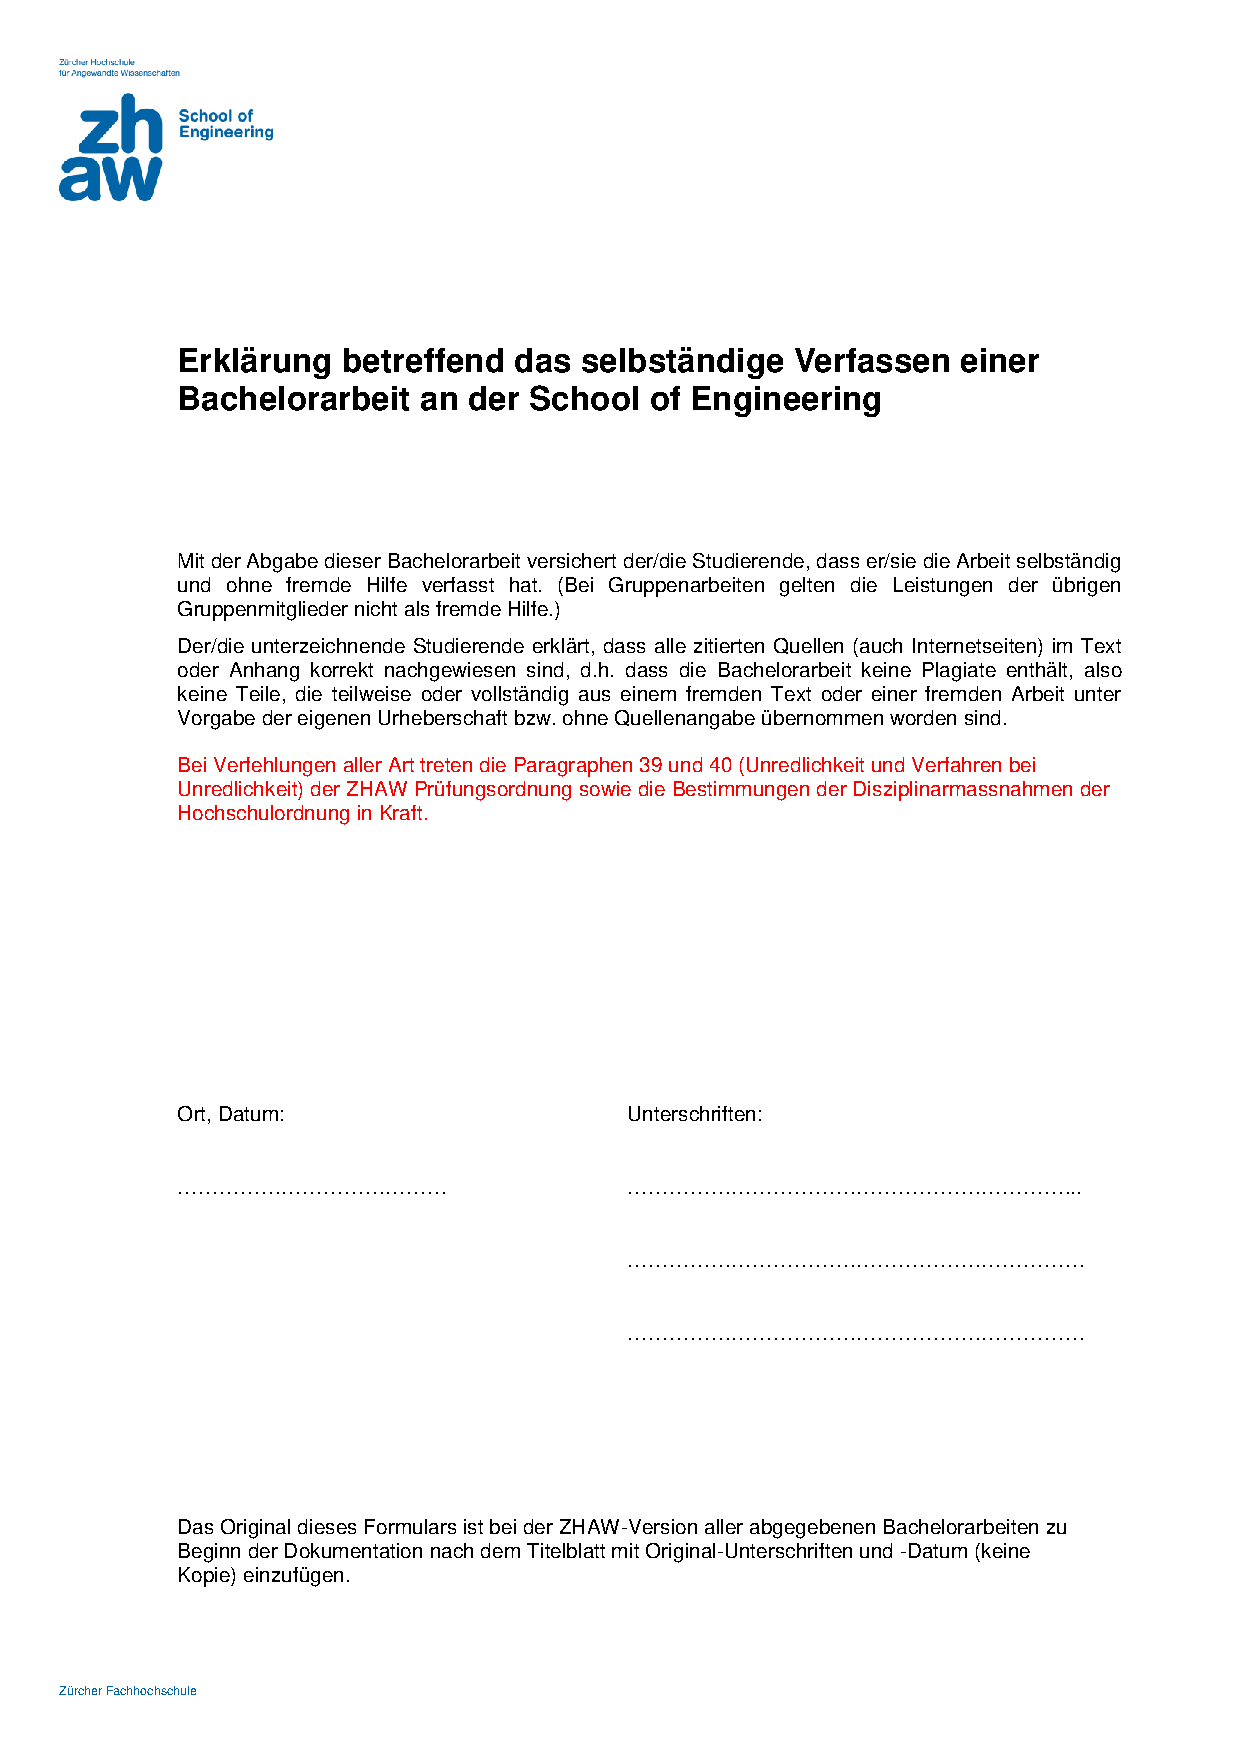
\includepdf{images/Erklaerung_BA.pdf} % Entsprechendes auskommentieren
% 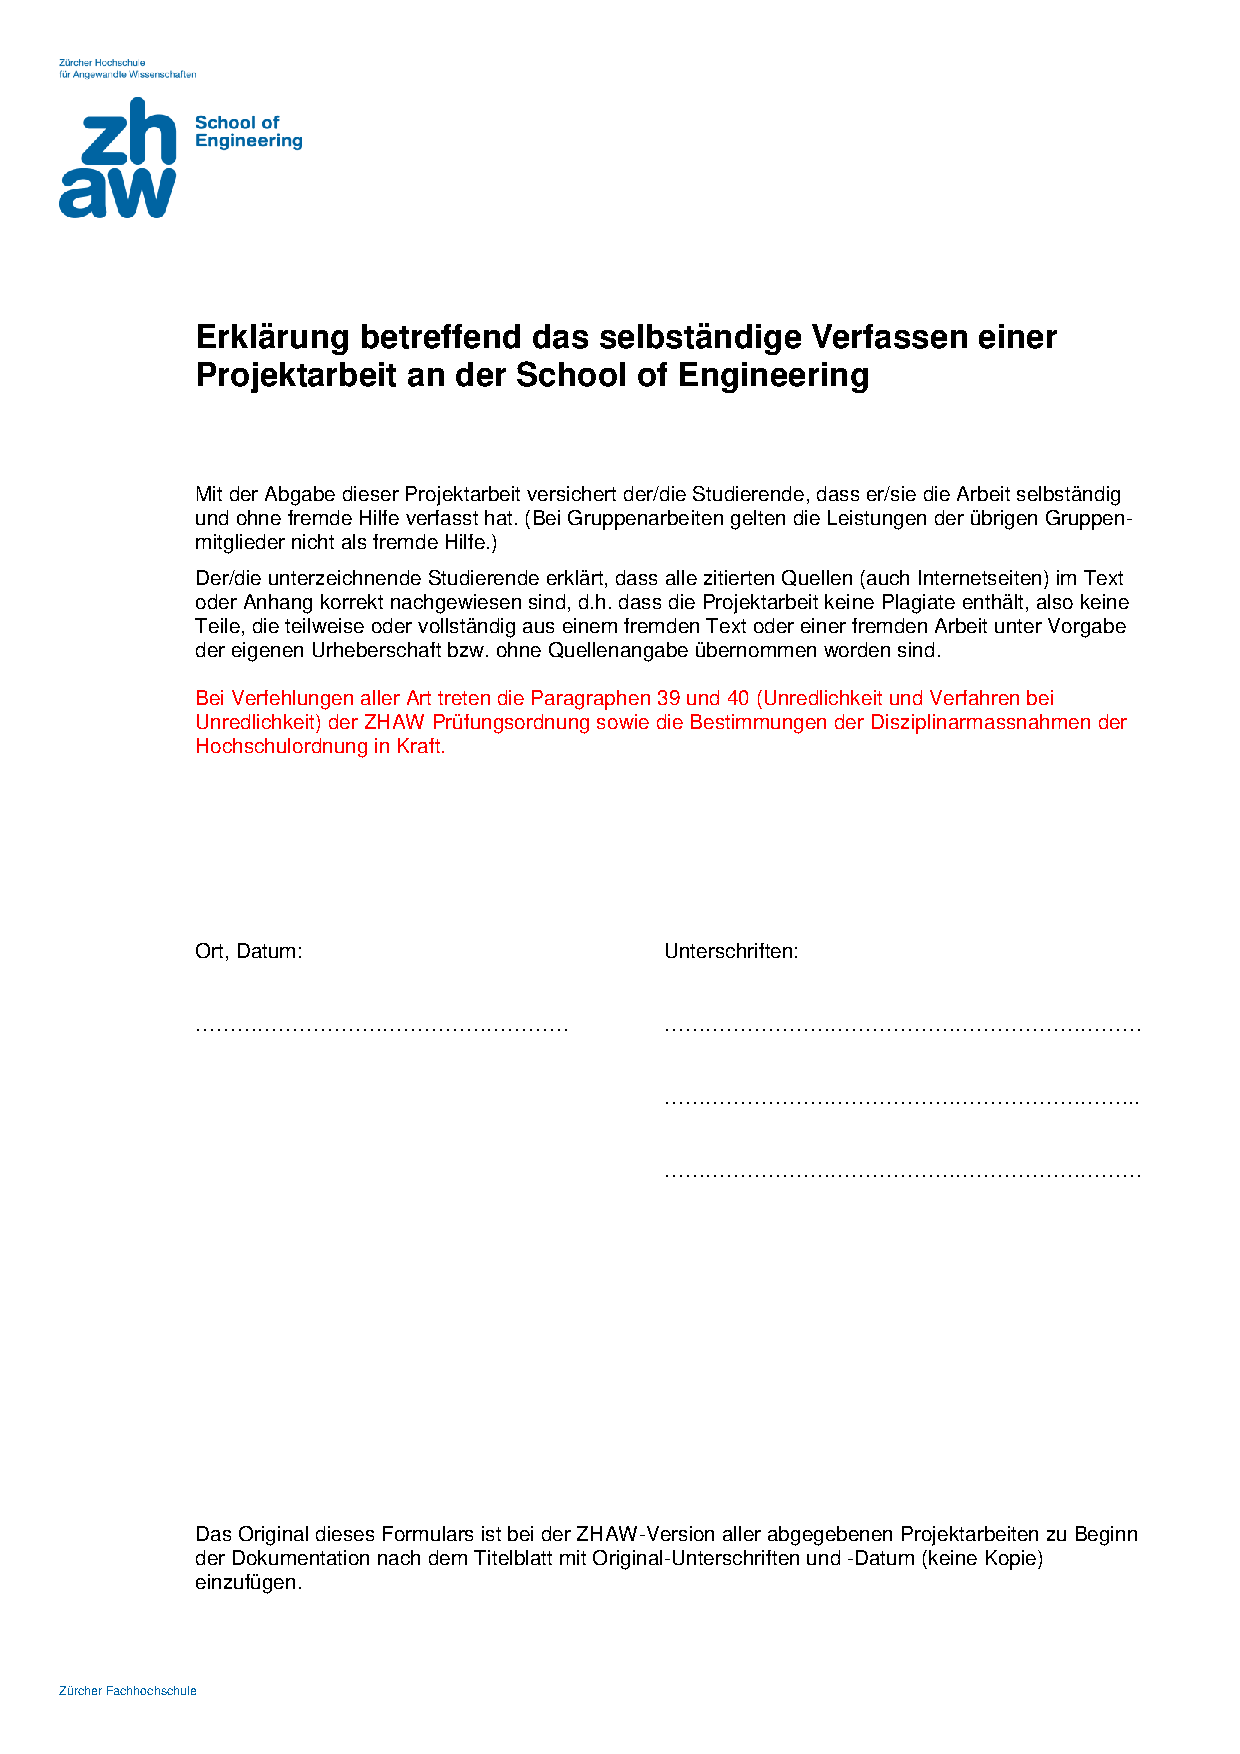
\includepdf{images/Erklaerung_PA.pdf}

\setcounter{page}{1}
%% !TeX spellcheck = de_CH
%%%%%%%%%%%%%%%%%%%%%%%%%%%%%%%%%%%%%%%%%%%%%%%%%%%%%%%%%%%%%%%%%
%  _____   ____  _____                                          %
% |_   _| /  __||  __ \    Institute of Computitional Physics   %
%   | |  |  /   | |__) |   Zuercher Hochschule Winterthur       %
%   | |  | (    |  ___/    (University of Applied Sciences)     %
%  _| |_ |  \__ | |        8401 Winterthur, Switzerland         %
% |_____| \____||_|                                             %
%%%%%%%%%%%%%%%%%%%%%%%%%%%%%%%%%%%%%%%%%%%%%%%%%%%%%%%%%%%%%%%%%
%
% Project     : Konzept BA Welti Keller
% Title       : 
% File        : Kontakt.tex Rev. 00
% Date        : 15.09.2014
% Author      : Tobias Welti
%
%%%%%%%%%%%%%%%%%%%%%%%%%%%%%%%%%%%%%%%%%%%%%%%%%%%%%%%%%%%%%%%%%

\textbf{Kontakte}


\textbf{Vorlagen Ersteller} \\
M.Sc. Engineering ZHAW Remo Ritzmann \\
Wissenschaftliche Assistent Optoelectronic Research Laboratory\\
School of Engineering\\
Technikumstrasse 9, TL419\\
CH-8408 Winterthur

Phone: +41 (0)52 534 48 62\\
Zentrale: +41 (0)58 934 73 06\\
Mobile: +41 (0)79 830 17 35\\
E-Mail: remo.ritzmann@zhaw.ch\\
E-Mail Privat: remo.ritzmann@pfunzle.ch\\
Homepage: \url{http://www.icp.zhaw.ch}\vskip 15pt



%Inhaltsverzeichnis
\tableofcontents
\newpage


%Kapitel
%\setcounter{page}{1}
%\pagenumbering{arabic}

% !TeX spellcheck = de_CH
%%%%%%%%%%%%%%%%%%%%%%%%%%%%%%%%%%%%%%%%%%%%%%%%%%%%%%%%%%%%%%%%%
%  _____   ____  _____                                          %
% |_   _| /  __||  __ \    Institute of Computitional Physics   %
%   | |  |  /   | |__) |   Zuercher Hochschule Winterthur       %
%   | |  | (    |  ___/    (University of Applied Sciences)     %
%  _| |_ |  \__ | |        8401 Winterthur, Switzerland         %
% |_____| \____||_|                                             %
%%%%%%%%%%%%%%%%%%%%%%%%%%%%%%%%%%%%%%%%%%%%%%%%%%%%%%%%%%%%%%%%%
%

% Project     : Pflichtenheft BA Welti Keller
% Title       : 
% File        : einleitung.tex Rev. 00
% Date        : 15.09.2014
% Author      : Tobias Welti
%
%%%%%%%%%%%%%%%%%%%%%%%%%%%%%%%%%%%%%%%%%%%%%%%%%%%%%%%%%%%%%%%%%

\chapter{Einleitung}\label{chap.einleitung}



\section{Ausgangslage}\label{sec.ausgangslage}
Die Eidg. Forschungsanstalt für Wald, Schnee und Landschaft (WSL) betreibt Messstationen zur Registrierung von Geschiebe-Bewegungen im Fluss mittels Geophonen, die unter Stahlplatten montiert sind. Diese Platten sind in einer Betonkonstruktion eingelassen, um sie im Flussbett zu fixieren. Die Geophone sind über Kabel mit einem Auswertungs-Rechner (Embedded PC) verbunden, der die Signale auswertet. Die baulichen Massnahmen für die Installation der Sensoren, der Auswertungsstation sowie der Stromversorgung sind sehr teuer. 


\section{Aufgabenstellung}\label{sec.aufgabenstellung}
Im Rahmen dieser Bachelorarbeit soll eine Lösung erarbeitet werden, um zukünftige Installationen günstiger zu machen. Da solche Messanlagen an sehr vielen Orten auf der ganzen Welt aufgebaut werden, kann durch eine Vereinfachung der Installation viel Aufwand gespart werden. 

Die Projektidee stammt von Bruno Fritschi (WSL). Sein Vorschlag sieht vor, die aufgezeichneten Signale direkt am Sensor auszuwerten und nur die gewünschten Ereignisse zu übertragen und zu speichern. Somit könnten die Daten über ein Bussystem übertragen werden und der Auswertungsrechner bräuchte weniger Leistung.

Dank der Bustopologie ist das Messsystem weniger komplex und kann einfacher installiert werden. Denkbar wäre die Integration in einer Gummimatte anstelle der Stahl- und Betonkonstruktion, da viel weniger Leitungen nötig sind.

Ziel der Arbeit ist die Entwicklung der Auswertungshardware und des Bussystems. Die Qualität der gemessenen Signale soll mindestens erhalten werden. Die Auswertungsalgorithmen sind nicht Bestandteil der Arbeit und werden vom WSL zur Verfügung gestellt.

Die von der bisherigen Anlage gemachten Messdaten enthalten die Dauer und Intensität jedes Aufschlags (Ereignis) auf der Sensorplatte, sowie die Anzahl Ausschläge (Peaks) pro Aufschlag. Pro Minute wird ein Histogramm über die Intesitäten der Peaks gebildet und abgespeichert.

Denkbar wäre es, einen Prototyp für Vergleichsmessungen im Erlenbach (Alptal, SZ) an einer bestehenden Schwelle zu implementieren.

\subsection{Musskriterien}
\begin{itemize}
\item Die Anlage zeichnet den Geschiebetransport im Bachbett auf. Die bisherige Aufzeichnungsrate von 10'000 Messpunkten pro Sekunde soll nicht unterschritten werden.
\item Die Anlage liefert eine minütliche Zusammenfassung über die Ereignisse an jedem Sensor. Diese Zusammenfassung enthält die Anzahl, Dauer und Intensität der einzelnen Ereignisse sowie ein Histogramm über die Intensitätsverteilung.
\item Die Messstation ist fähig, mindestens zehn Sensoren zu betreiben und ihre Messignale aufzuzeichnen.
\item Es ist möglich, die kompletten Rohdaten von einem Sensor über eine Dauer von 30 Minuten aufzuzeichnen. Während einer solchen Messung dürfen die anderen Sensoren ihre Messung einstellen.
\item Die Sensoren können über bis zu fünfzehn Meter im Bachbett verteilt sein.
\item Die Leistungsaufnahme der Anlage beim Betrieb von 10 Sensoren ist kleiner als zehn Watt.
\item Die Datenaufzeichnung erfolgt in einem eigens entwickelten Datenlogger.
\item Am Datenlogger kann ein Laptop angeschlossen werden, um Kontrollparameter der Messanlage zu setzen und um den Status der Anlage abzufragen.
\item Die erfassten Messdaten werden im Datenlogger auf einer Speicherkarte gespeichert. Dies ermöglicht ein einfaches Abholen der Daten im Feld, indem die Speicherkarte ausgetauscht wird.
\end{itemize}
\subsection{Wunschkriterien}
\begin{itemize}
\item Die Anlage liefert für jedes Ereignis die Rohdaten in voller zeitlicher Auflösung.
\item Der Sensoraufbau ermöglicht es, die Sensoren in einer Elastomerplatte zu verpacken. Die Elastomerplatte kann ohne Betonkonstruktion im Bachbett verankert werden.
\item Am Datenlogger kann ein Laptop angeschlossen werden, um die erfassten Messdaten herunterzuladen.
\end{itemize}
\subsection{Abgrenzungskriterien}
\begin{itemize}
\item Es würde den Rahmen dieser Arbeit sprengen, die Messeinheiten zur Produktreife zu bringen. Es wird lediglich aufgezeigt, wie solche Messeinheiten realisiert werden könnten.
\item Eine Testinstallation in einem Bach ist nicht möglich. Allenfalls kann in der Versuchsanstalt für Wasserbau, Hydrologie und Glaziologie der ETH Zürich ein kleiner Testlauf stattfinden.
\item
\end{itemize}

% !TeX spellcheck = de_CH
% !TeX spellcheck = de_CH
%%%%%%%%%%%%%%%%%%%%%%%%%%%%%%%%%%%%%%%%%%%%%%%%%%%%%%%%%%%%%%%%%
%  _____   ____  _____                                          %
% |_   _| /  __||  __ \    Institute of Computational Physics   %
%   | |  |  /   | |__) |   Zuercher Hochschule Winterthur       %
%   | |  | (    |  ___/    (University of Applied Sciences)     %
%  _| |_ |  \__ | |        8401 Winterthur, Switzerland         %
% |_____| \____||_|                                             %
%%%%%%%%%%%%%%%%%%%%%%%%%%%%%%%%%%%%%%%%%%%%%%%%%%%%%%%%%%%%%%%%%
%
% Project     : BA Welti Keller
% Title       : 
% File        : funktionale.tex Rev. 00
% Date        : 15.09.2014
% Author      : Tobias Welti
%
%%%%%%%%%%%%%%%%%%%%%%%%%%%%%%%%%%%%%%%%%%%%%%%%%%%%%%%%%%%%%%%%%

\thispagestyle{empty}
\chapter{Funktionale Anforderungen}\label{chap.funktionale}
\section{\gls{logger} (F1\ldots)}


\subsection{F110 Busmaster}
Der \gls{logger} übernimmt die Kontrolle des \gls{bussys}. Bei Inbetriebnahme des Systems tastet der \gls{logger} den Bus nach \glspl{sensoreinh} ab und erteilt jeder \gls{sensoreinh} eine eindeutige Identifikationsnummer (ID). Die ID des \gls{logger}s soll so gewählt werden, dass er jederzeit Priorität hat, auf den Bus zu schreiben.


\subsection{F120 Sensorerkennung}
Die angeschlossenen \glspl{sensor} werden vom \gls{logger} erkannt und mit einer ID versehen. Anhand der ID wird die Priorität bei der Datenübertragung festgelegt und der \gls{sensor} identifiziert. Ein Sensor, der bereits am System angeschlossen war, erhält wieder die gleiche \gls{id}, sofern die Konfigurationsdatei nicht gelöscht wurde.


\subsection{F130 Uhrzeit}
Der \gls{logger} verfügt über eine interne Uhr, um die \glspl{ereignis} in den Dateien mit einem lesbaren Zeitstempel zu versehen.


\subsection{F140 \gls{timestamp} verteilen}
Der \gls{logger} sendet ein Signal an alle \glspl{sensoreinh}, dass der Zeitstempel (\gls{timestamp}) neu gestellt werden soll. Ab dann beziehen sich die \gls{timestamp}s auf die Dauer seit dem jetzigen Zeitpunkt.


\subsection{F160 Schnittstelle zum Steuerrechner}
Der \gls{logger} bietet eine Schnittstelle, an der ein Steuerrechner (Laptop, \gls{pc}) angeschlossen werden kann. Über diese Schnittstelle kann der Betrieb der ganzen Anlage gesteuert werden.


\subsection{F170 Steuerung Betriebsmodus}
Der Betriebsmodus der \glspl{sensor} wird vom \gls{logger} aus gesteuert: Wie viele und welche Art von Daten gesammelt werden soll und ob alle \glspl{sensor} oder nur bestimmte aktiv sein sollen. \\
Folgende Betreibsmodi sind verfügbar:
\begin{itemize}
\item Normaler Modus: Alle \glspl{sensor} übermitteln die verarbeiteten Ereignisdaten. Zeitpunkt, Intensität, Dauer und Anzahl Ausschläge jedes \gls{ereignis} werden gespeichert.
\item Detaillierter Modus: Alle \glspl{sensor} übermitteln die verarbeiteten Ereignisdaten sowie die gesamten Messdaten für die Dauer des \gls{ereignis}.
\item Rohdatenmodus: Ein \gls{sensor} übermittelt kontinuierlich Rohdaten, die anderen \glspl{sensor} werden vorübergehend abgeschaltet.
\end{itemize}


\subsection{F180 Daten sammeln}
Der \gls{logger} fragt in regelmässigen Abständen bei den \glspl{sensoreinh} an, ob Ereignisdaten zur Übertragung bereit sind. Diese übermitteln die vorliegenden Ereignisdaten.


\subsection{F190 Daten speichern}
Die Daten werden vom \gls{logger} auf einer Speicherkarte in Dateien abgelegt. Nach entsprechenden Befehlen vom Steuerrechner kann die Karte entfernt und ausgetauscht werden, um die Daten abzuholen.


\section{\gls{sensoreinh} (F4\ldots)}


\subsection{F410 Ereignisdetektion}
Die \gls{sensoreinh} liest den \gls{sensor} mit einer definierten \gls{fs} aus und wertet die Messdaten aus. Der Prozessor erkennt \glspl{ereignis} anhand definierter Kriterien. Zu jedem \gls{ereignis} werden folgende Daten gespeichert: Zeitpunkt (\gls{timestamp}), Dauer, Anzahl Peaks und höchster Peak. In einem zweiten Betriebsmodus können alle Messpunkte während einem \gls{ereignis} gespeichert werden.


\subsection{F430 Datenübertragung}
Die \gls{sensoreinh} übermittelt die Ereignisdaten über das \gls{bussys} an den \gls{logger}.


\subsection{F450 Rohdatenaufzeichnung}
In einem Sondermodus werden alle Messpunkte gespeichert und über das \gls{bussys} an den \gls{logger} übertragen. In diesem Betriebsmodus kann darf auch nur eine \gls{sensoreinh} aktiv sein, die anderen werden auf Standby geschaltet.



% %%%%%%%%%%%%%%%%%%%%%%%%%%%%%%%%%%%%%%%%%%%%%%%%%%%%%%%%%%%%%%%%%
%  _____   ____  _____                                          %
% |_   _| /  __||  __ \    Institute of Computitional Physics   %
%   | |  |  /   | |__) |   Zuercher Hochschule Winterthur       %
%   | |  | (    |  ___/    (University of Applied Sciences)     %
%  _| |_ |  \__ | |        8401 Winterthur, Switzerland         %
% |_____| \____||_|                                             %
%%%%%%%%%%%%%%%%%%%%%%%%%%%%%%%%%%%%%%%%%%%%%%%%%%%%%%%%%%%%%%%%%
%
% Project     : Pflichtenheft BA Welti Keller
% Title       : 
% File        : funktionsbaum.tex Rev. 0
% Date        : 15.09.2014
% Author      : Tobias Welti
%
%%%%%%%%%%%%%%%%%%%%%%%%%%%%%%%%%%%%%%%%%%%%%%%%%%%%%%%%%%%%%%%%%

\thispagestyle{empty}
\chapter{Funktionsbaum}\label{sec.funktionsbaum}

% !TeX spellcheck = de_CH
%%%%%%%%%%%%%%%%%%%%%%%%%%%%%%%%%%%%%%%%%%%%%%%%%%%%%%%%%%%%%%%%%
%  _____   ____  _____                                          %
% |_   _| /  __||  __ \    Institute of Computitional Physics   %
%   | |  |  /   | |__) |   Zuercher Hochschule Winterthur       %
%   | |  | (    |  ___/    (University of Applied Sciences)     %
%  _| |_ |  \__ | |        8401 Winterthur, Switzerland         %
% |_____| \____||_|                                             %
%%%%%%%%%%%%%%%%%%%%%%%%%%%%%%%%%%%%%%%%%%%%%%%%%%%%%%%%%%%%%%%%%
%
% Project     : Pflichtenheft BA Welti Keller
% Title       : 
% File        : nichtfunktionale.tex Rev. 00
% Date        : 15.09.2014
% Author      : Tobias Welti
%
%%%%%%%%%%%%%%%%%%%%%%%%%%%%%%%%%%%%%%%%%%%%%%%%%%%%%%%%%%%%%%%%%

\thispagestyle{empty}
\chapter{Nichtfunktionale Anforderungen}\label{chap.nichtfunktionale}

\begin{itemize}
\item Die gesamte Messstation soll eine geringere Leistungsaufnahme haben als eine aktuelle Messstation mit Geophonen. Für zehn Geophone sind dies zur Zeit zehn Watt.

\item Die Installation soll weniger bauliche Massnahmen erfordern als eine aktuelle Messstation mit Geophonen.

\item Die erfassten Ereignisdaten sollen mehr Details enthalten als mit den bisherigen Installationen.

\item Sensoreinheiten müssen wasserdicht verpackt werden können.
\
\end{itemize}
%%%%%%%%%%%%%%%%%%%%%%%%%%%%%%%%%%%%%%%%%%%%%%%%%%%%%%%%%%%%%%%%%
%  _____   ____  _____                                          %
% |_   _| /  __||  __ \    Institute of Computitional Physics   %
%   | |  |  /   | |__) |   Zuercher Hochschule Winterthur       %
%   | |  | (    |  ___/    (University of Applied Sciences)     %
%  _| |_ |  \__ | |        8401 Winterthur, Switzerland         %
% |_____| \____||_|                                             %
%%%%%%%%%%%%%%%%%%%%%%%%%%%%%%%%%%%%%%%%%%%%%%%%%%%%%%%%%%%%%%%%%
%
% Project     : LaTeX doc Vorlage für Windows ProTeXt mit TexMakerX
% Title       : 
% File        : abstract.tex Rev. 00
% Date        : 23.4.12
% Author      : Remo Ritzmann
% Feedback bitte an Email: remo.ritzmann@pfunzle.ch
%
%%%%%%%%%%%%%%%%%%%%%%%%%%%%%%%%%%%%%%%%%%%%%%%%%%%%%%%%%%%%%%%%%

\thispagestyle{empty}
\chapter{Abnahmekriterien}\label{chap.abnahme}
Die Abnahmekriterien sind in den Kapiteln 

\chapter{Verzeichnisse}\label{chap.verzeichnisse}
 %%%%%%%%%%%%%%%%%%%%%%%%%%%%%%%%%%%%%%%%%%%%%%%%%%%%%%%%%%%%%%%%%
%  _____   ____  _____                                          %
% |_   _| /  __||  __ \    Institute of Computitional Physics   %
%   | |  |  /   | |__) |   Zuercher Hochschule Winterthur       %
%   | |  | (    |  ___/    (University of Applied Sciences)     %
%  _| |_ |  \__ | |        8401 Winterthur, Switzerland         %
% |_____| \____||_|                                             %
%%%%%%%%%%%%%%%%%%%%%%%%%%%%%%%%%%%%%%%%%%%%%%%%%%%%%%%%%%%%%%%%%
%
% Project     : LaTeX doc Vorlage für Windows ProTeXt mit TexMakerX
% Title       : 
% File        : literatur.tex Rev. 00
% Date        : 23.4.12
% Author      : Remo Ritzmann
% Feedback bitte an Email: remo.ritzmann@pfunzle.ch
%
%%%%%%%%%%%%%%%%%%%%%%%%%%%%%%%%%%%%%%%%%%%%%%%%%%%%%%%%%%%%%%%%%

\begin{thebibliography}{99}
\addcontentsline{toc}{section}{Literaturverzeichnis}\label{cha:literaturverzeichnis}

% How to make a Literaturlist nach www.ieee.org/documents/ieeecitationref.pdf
% Erklärung

%Books
\bibitem{robotvision} B. Klaus and P. Horn, Robot Vision. Cambridge, MA: MIT Press, 1986.
%Einzelne Seiten aus Buch
\bibitem{randompatterns} L. Stein, ">Random patterns,"> in Computers and You, J. S. Brake, Ed. New York: Wiley, 1994, pp. 55-70.



\end{thebibliography}

 \listoffigures
 \addcontentsline{toc}{section}{(Abbildungsverzeichnis)}
 \listoftables
 \addcontentsline{toc}{section}{(Tabellenverzeichnis)}
% \addcontentsline{toc}{chapter}{(Symbolverzeichnis)}
 % !TeX spellcheck = de_CH
%%%%%%%%%%%%%%%%%%%%%%%%%%%%%%%%%%%%%%%%%%%%%%%%%%%%%%%%%%%%%%%%%
%  _____   ____  _____                                          %
% |_   _| /  __||  __ \    Institute of Computitional Physics   %
%   | |  |  /   | |__) |   Zuercher Hochschule Winterthur       %
%   | |  | (    |  ___/    (University of Applied Sciences)     %
%  _| |_ |  \__ | |        8401 Winterthur, Switzerland         %
% |_____| \____||_|                                             %
%%%%%%%%%%%%%%%%%%%%%%%%%%%%%%%%%%%%%%%%%%%%%%%%%%%%%%%%%%%%%%%%%
%
% Project     : BA Welti Keller
% Title       : 
% File        : glossar.tex Rev. 00
% Date        : 15.09.2014
% Author      : Tobias Welti
%
%%%%%%%%%%%%%%%%%%%%%%%%%%%%%%%%%%%%%%%%%%%%%%%%%%%%%%%%%%%%%%%%%

% Abkürzungen
\newacronym{wsl}{WSL}{Eidg. Forschungsanstalt für Wald, Schnee und Landschaft}

\newacronym{vaw}{VAW}{Versuchsanlage für Wasserbau}

\newacronym{id}{ID}{Identifikationsnummer}

\newacronym{pc}{PC}{Personal Computer}

\newacronym{cpu}{CPU}{Central Processing Unit}

\newacronym{cd}{CD}{Compact Disc}

\newacronym{adc}{ADC}{Analog Digital Converter}

\newacronym{dft}{DFT}{dis\-kre\-te Fou\-rier-Trans\-for\-ma\-tion}

\newacronym{idft}{IDFT}{inverse diskrete Fourier-Transformation}

\newacronym{fsm}{FSM}{Finite State Machine}

\newacronym{dsp}{DSP}{Digitaler Signal-Prozessor}

\newacronym{nvic}{NVIC}{Nested Vectored Interrupt Controller}

\newacronym{mac}{MAC}{multiply-accumulate unit}

\newacronym{fpu}{FPU}{Floating Point Unit}

\newacronym{isr}{ISR}{Interrupt Service Routine}

\newacronym{cdet}{CD}{Collision Detection}

\newacronym{mcacr}{MC}{Microkontroller}

\newacronym{crc}{CRC}{Cyclic Redundancy Check}

\newacronym{usb}{USB}{Universal Serial Bus}

\newacronym{mci}{MCI}{Memory Card Interface}

\newacronym{irq}{IRQ}{Interrupt Request}

% Glossareinträge
\newglossaryentry{geophon}{name={Geophon},plural={Geophone},description={Ein Messgerät für Vibrationen des Bodens. Ein Geophon misst Bewegungen mittels einer magnetischen Masse, die beweglich in einer Spule aufgehängt ist. Wird das Geophon in Bewegung versetzt, schwingt die magnetische Masse aufgrund ihrer Trägheit und induziert dadurch einen Strom in der Spule. Durch Messung dieses Stroms kann die Bewegung registriert werden.}}


\newglossaryentry{logger}{name={Datenlogger},plural={Datenlogger},description={Ein Gerät zur Sammlung und Speicherung von Messdaten von mehreren Sensoreinheiten.}, see={sensoreinh}}

\newglossaryentry{speichermedium}{name={Speichermedium},plural={Speichermedien},description={Ein Stück Hardware, auf dem Daten gespeichert werden können.}}

\newglossaryentry{sensoreinh}{name={Sensoreinheit},plural={Sensoreinheiten},description={Ein kombiniertes elektronisches Gerät zur Messung von physikalischen Daten und der Verarbeitung dieser Daten. Das Gerät verfügt über einen Mikroprozessor und einen Sensor. Optional kann auch eine Schnittstelle für die Kommunikation mit einem Datenlogger vorhanden sein.},see={mc,sensor,logger}}

\newglossaryentry{sensor}{name={Sensor},plural={Sensoren},description={Ein Messgerät für physikalische Grössen wie Temperatur, Feuchtigkeit, Luftdruck oder Beschleunigung.}}

\newglossaryentry{bussys}{name={Bussystem},plural={Bussysteme},description={Ein elektrisches System für die Kommunikation zwischen mehreren Geräten. Ein Bussystem besteht aus Datenleitungen, über welche Signale gesendet werden, und aus Schnittstellen, an denen die Busteilnehmer angeschlossen werden. Die Besonderheit liegt darin, dass über ein Leitungssystem mehr als zwei Geräte miteinander kommunizieren können. Mittels eines Adressierungsschemas können die Empfänger ausgewählt werden.},see={signal}}

\newglossaryentry{ereignis}{name={Ereignis},plural={Ereignisse},description={Eine Abfolge von Messwerten, die einer vordefinierten Form entspricht. Es kann zum Beispiel ein Schwellenwert (engl. threshold) definiert sein. Das Überschreiten dieses Wertes kann dann den Beginn, das Unterschreiten des Schwellenwertes das Ende eines Ereignisses markieren.}}

\newglossaryentry{ereignisdet}{name={Er\-eig\-nis\-er\-ken\-nung},plural={Ereigniserkennungen},description={Auswertung von Messdaten um definierte Signalformen (\glspl{ereignis}) zu erkennen.},see={ereignis,signal}}

\newglossaryentry{threshold}{name={Threshold},plural={Thresholds},description={Englisch für Schwellenwert.}}

\newglossaryentry{timeout}{name={Timeout},plural={Timeouts},description={Englisch für Zeitüberschreitung.}}

\newglossaryentry{peak}{name={Peak},plural={Peaks},description={Englisch für Spitzenwert oder Signalspitze.}}

\newglossaryentry{signal}{name={Signal},plural={Signale},description={Ein Signal ist ein Informationsträger. Die Information wird einem Signalwert zugeordnet. Ein einfaches Beispiel ist die Spannung am Ausgang eines Beschleunigungs-Sensors. Der Sensor gibt über die Höhe der Spannung an, wie stark die Beschleunigung von einem definierten Referenzwert abweicht. Die Spannung trägt also eine Information über den Messwert und ist daher ein Signal. Aus dem Datenblatt kann herausgelesen werden, wie hoch die ausgegebene Spannung bei einer bestimmten Beschleunigung ist. So kann das Signal in Information umgewandelt werden.},see={sensor}}

\newglossaryentry{timestamp}{name={Timestamp},plural={Timestamps},description={Englisch für Zeitmarke. Mittels eines Timestamps kann ein Ereignis oder ein Messwert einem genauen Zeitpunkt zugeordnet werden. Der Timestamp wird dafür zu einem bestimmten Zeitpunkt auf null gesetzt (Reset) und in allen Messgeräten in vordefiniertem Takt erhöht. Der Timestamp gibt an, wie viel Zeit seit dem Reset vergangen ist. Durch die Wahl des Takts wird die zeitliche Auflösung definiert.}}

\newglossaryentry{compi}{name={Computer},description={Englisch für Elektronenrechner. Unter einem Computer versteht man umgangssprachlich einen Personal Computer (PC) oder einen tragbaren Computer (Laptop). Heute sind Computer so leistungsfähig und so stark miniaturisiert, dass sie mühelos in einer Aktentasche Platz finden. Weniger leistungsfähig, dafür noch kleiner sind Embedded Systems, eingebettete Systeme, die von Laien nicht als Computer erkannt werden.},see={pc,es}}

\newglossaryentry{pcomp}{name={PC},plural={PCs},description={\gls{pc} oder umgangssprachlich Computer. Eine elektronische Rechenmaschine mit der sehr viele Rechenschritte in sehr kurzer Zeit ausgeführt werden können. Mit der richtigen Programmierung (Software) können \gls{pc}s sehr unterschiedliche, umfangreiche Aufgaben lösen.},see={software}}

\newglossaryentry{es}{name={Embedded System},plural={Embedded Systems},description={Deutsch: eingebettetes System. Ein Computer, der nicht über die üblichen Ein- und Ausgabemöglichkeiten eines Computers wie Bildschirm und Tastatur verfügt. Oft werden deshalb Embedded Systems nicht als Computer wahrgenommen. Sie sind im Gegensatz zu PCs, die als Alleskönner konzipiert sind, auf eine bestimmte Aufgabe zugeschnitten und deshalb nur mit den nötigen Bedien-Elementen versehen. Oft genügen für die Aufgaben weniger leistungsfähige Prozessoren als in einem PC, sogenannte Mikroprozessoren.},see={compi,mc}}

\newglossaryentry{software}{name={Software},description={Programm zur Steuerung der Rechenabläufe in einem Computer. Durch die Software wird einem Computer die Fähigkeit gegeben, bestimmte Aufgaben zu lösen und Resultate in einer für Menschen lesbaren Form darzustellen. Die Software enthält Instruktionen, die in der CPU des Computers ausgeführt werden.}}

\newglossaryentry{hardware}{name={Hardware},description={Die Hardware ist das eigentliche Rechenwerk eines Computers, worauf die Software ausgeführt wird. Dazu gehören alle elektrischen, elektronischen und mechanischen Bauteile eines Computers. Die Central Processing Unit (CPU) eines Computers könnte mit dem Hirn verglichen werden, hier laufen fast sämtliche Informationen und Instruktionen zusammen.}}

\newglossaryentry{mc}{name={Mikrokontroller},plural={Mikrokontroller},description={Englisch Microcontroller (MC). Ein Prozessor mit weniger universellen Fähigkeiten als eine CPU, mit entsprechend geringerem Stromverbrauch. Ein Mikrokontroller verfügt meistens über spezielle Ein- und Ausgänge (Pins), über die zum Beispiel die anliegende Spannung gemessen oder eine bestimmte Spannung ausgegeben werden kann. Durch die kleinere Bauform und die geringere Leistungsaufnahme eignen sich diese Prozessoren besonders für den Einsatz in Embedded Systems, die oft längere Zeit unabhängig vom Stromnetz funktionieren müssen.},see={pin}}

\newglossaryentry{cli}{name={Kommandozeile},plural={Kommandozeilen},description={Eine Eingabeaufforderung auf dem Bildschirm, wo der Benutzer über eine Tastatur Befehle eingeben kann, die vom Computer interpretiert und ausgeführt werden.},see={compi}}

\newglossaryentry{pin}{name={Pin},plural={Pins},description={Ein Anschluss an einem Chip oder einer Leiterplatte. Über Pins werden elektronische Bauteile miteinander verbunden und Peripheriegeräte wie z.B. Sensoren angeschlossen.},see={sensor}}

\newglossaryentry{modus}{name={Betriebsmodus},plural={Betriebsmodi},description={Ein Modus bestimmt die Verhaltensweise eines Systems. Je nach gewähltem Modus können mit den gleichen Eingaben und Befehlen andere Aktionen ausgeführt und andere Resultate ausgegeben werden.}}

\newglossaryentry{fs}{name={Abtastrate},plural={Abtastraten},description={Definiert, in welchen zeitlichen Abständen ein Messwert erfasst werden soll. Üblicherweise wird dieser Wert in \ensuremath{Hz} oder \ensuremath{s^{-1}} angegeben.}}

\newglossaryentry{busmaster}{name={Busmaster},plural={Busmaster},description={Ein Gerät, das die Kontrolle über ein Bussystem hat. Der Busmaster kann den anderen Busteilnehmern (Slaves) eine Genehmigung erteilen, Daten über das Bussystem zu übertragen. Der Busmaster hat aber jederzeit die Möglichkeit, einen Slave in der Übertragung zu unterbrechen.},see={slave}}

\newglossaryentry{slave}{name={Slave},plural={Slaves},description={Ein Busteilnehmer, der nur Daten über den Bus übertragen darf, wenn ihm der Busmaster die Genehmigung dafür erteilt. Dies kann z.B. in Form eines sog. Tokens geschehen.},see={busmaster}}

\newglossaryentry{adwandler}{name={A/D-Wandler},plural={A/D-Wandler},description={Analog/Digital-Wandler, (Englisch: \gls{adc}). Ein A/D-Wandler misst die Spannung, die an einem Pin anliegt und gibt einen digitalen Wert aus, der die Höhe der Spannung angibt. Bei der Umwandlung in einen digitalen Wert erfolgt eine Quantisierung. Je grösser die Bit-Breite des A/D-Wandlers ist, umso kleiner wird die Schrittgrösse von einem digitalen Wert zum nächst höheren Wert.},see={quantis,bitbreite}}

\newglossaryentry{quantis}{name={Quantisierung},plural={Quantisierung},description={Einteilung eines Werts aus einer kontinuierlichen Skala in eine abgestufte Skala. Bei der Quantisierung wird der nächstgelegene Wert auf der abgestuften Skala ausgewählt. Je nach Anwendung wird die abgestufte Skala mit konstanter Stufengrösse (linear) gewählt, oder mit unterschiedlichen Stufengrössen je nach absolutem Wert (z.B. exponentiell). Der Quantisierungsfehler entspricht der Differenz zwischen dem analogen und dem quantisierten, digitalen Wert. Je grösser die Bit-Breite der Quantisierung ist, desto kleiner wird der Quantisierungsfehler.},see={bitbreite}}

\newglossaryentry{bitbreite}{name={Bit-Breite},plural={Bit-Breiten},description={Die Bit-Breite gibt an, wie viele Bit für die Darstellung eines Wertes verwendet werden. Je grösser die Bit-Breite, desto mehr unterschiedliche Werte können dargestellt werden. Mit einer Bit-Breite von \ensuremath{n} können \ensuremath{2^n} Werte dargestellt werden.}}

\newglossaryentry{blockg}{name={Blockgrösse},plural={Blockgrössen},description={Anzahl Werte, die in einer \gls{dft} oder \gls{idft} verrechnet wird.}}

\newglossaryentry{hilbert}{name={Hilbert-Transformation},plural={Hilbert-Transformationen},description={Mathematische Umrechnung einer Wertfolge, um die umhüllende Kurve zu erhalten.}}

\newglossaryentry{fir}{name={FIR-Filter},plural={FIR-Filter},description={Finite Impulse Response, Englisch für Filter mit endlicher Impuls-Antwort. Ein FIR-Filter hat immer eine endliche Impulsantwort, d.h. auf einen kurzen Impuls am Eingang des Filters folgt am Ausgang eine Antwort des Filters, die garantiert endet. Die Ordnung des FIR-Filters gibt an, wie lange die Antwort dauern wird.}}

\newglossaryentry{fsmgloss}{name={Finite State Machine},description={Englisch für Zustandsmaschine. Eine Finite State Machine definiert eine endliche Anzahl Zustände, die die Maschine einnehmen kann. Die \gls{fsm} reagiert auf Ereignisse, indem sie Aktionen auslöst und allenfalls in einen anderen Zustand wechselt. Für jeden Zustand ist definiert, welche möglichen Ereignisse welche Aktionen auslösen, und in welchen Folgezustand gewechselt werden soll.}}

\newglossaryentry{nullpegel}{name={Nullpegel},description={Signalpegel, wenn keine Beschleunigung gemessen wird.}}

\newglossaryentry{queue}{name={Queue},plural={Queues},description={Englisch für Warteschlange. In der Informationstechnologie wird eine Queue verwendet, um mehrere Werte zwischenzuspeichern, bis sie verarbeitet werden können. Eine Queue hat meistens eine vordefinierte Grösse und kann deshalb nur eine bestimmte Anzahl Werte aufnehmen. Ein Überlaufen der Queue hat einen Datenverlust zur Folge, wenn der Werte einfüllende Prozess nicht angehalten werden kann/darf, bis Platz in der Queue vorhanden ist.}}

\newglossaryentry{dspgloss}{name={DSP},plural={DSP},description={Digitaler Signal-Prozessor. Ein Mikroprozessor oder ein Bestandteil eines solchen, der dank spezieller Hardware fähig ist, Multiplikationen und Additionen extrem schnell auszuführen. Ausserdem verfügt ein \gls{dsp} über Schieberegister, um Rechenoperationen über eine Serie der aktuellsten Messwerte auszuführen. Da bei der digitalen Signalverarbeitung oft für jeden Messwert viele Multiplikations- und Additions-Schritte ausgeführt werden müssen, ist es wichtig, dass Multiplikations-Operationen in einem Taktzyklus ausgeführt werden können. In einem normalen Prozessor werden für eine Multiplikation mehrere Taktzyklen benötigt.},see={mc}}

\newglossaryentry{nvicgloss}{name={Nested Vectored Interrupt Controller},description={Wird benötigt, um möglichst rasch auf mehrere asynchron eintreffende Ereignisse reagieren zu können. Ein Prozessor mit NVIC kann auf verschiedene Ereignisse reagieren, indem Interrupts ausgelöst werden. Jedem Interrupt kann eine Priorität zugewiesen werden, um festzulegen, ob ein Interrupt einen anderen unterbrechen darf, der gerade vom Prozessor abgearbeitet wird.},see={interrupt}}

\newglossaryentry{macgloss}{name={MAC},description={Multiply-ACcumulate unit: Ein Rechenwerk in der CPU, wo Multiplikationen und Additionen ausgeführt werden.}}

\newglossaryentry{fpugloss}{name={FPU},description={Floating Point Unit, ein Rechenwerk in der CPU, die Berechnungen mit Dezimalbrüchen sehr schnell ausführen kann.}}

\newglossaryentry{sdram}{name={SDRAM},description={Synchronous Dynamic RAM. Flüchtiger Arbeitsspeicher. Der Inhalt des Arbeitsspeichers muss regelmässig aufgefrischt werden, sonst geht die Information verloren.},see={RAM}}

\newglossaryentry{flash}{name={Flash-Speicher},description={Nicht-flüchtiger Speicher. Der Inhalt des Speichers bleibt auch bestehen, wenn keine Versorgungsspannung anliegt.}}

\newglossaryentry{ram}{name={RAM},description={Random Access Memory. Arbeitsspeicher mit Zugriff auf beliebige Adressen. Benötigt keine Positionierung eines Lese-/Schreib-Kopfs oder eines Magnetbands vor einem Zugriff.}}

\newglossaryentry{polling}{name={Polling},description={Englisch für Abfragen. Bezeichnet das wiederholte Abfragen einer Funktion oder eines Wertes, bis ein bestimmtes Ereignis auftritt. Der Prozessor ist mit der Abfrage beschäftigt und verliert dadurch Rechenzeit.}}

\newglossaryentry{interrupt}{name={Interrupt},plural={Interrupts},description={Englisch für Unterbrechen. Durch ein spezielles Signal wird dem Prozessor mitgeteilt, dass ein Ereignis eingetreten ist. Der Prozessor unterbricht die laufende Funktion und ruft eine spezielle Routine, die \gls{isr} auf. Die \gls{isr} verarbeitet das Ereignis und gibt danach die Kontrolle an die vorher unterbrochene Funktion zurück. Mit einem Interrupt wird zwar die Abarbeitung einer Funktion kurzzeitig unterbrochen, dafür verliert der Prozessor keine Rechenzeit mit Polling.},see={polling}}

\newglossaryentry{cdetgloss}{name={Collision Detection},description={Kollisionserkennung. Als Kollision bezeichnet man den gleichzeitigen Versuch mehrerer Busteilnehmer, eine Nachricht zu übermitteln. Dies führt zu einer Überlagerung der Nachrichten und macht diese unlesbar. Gleichzeitig mit dem Schreiben liest der Transceiver die Signale vom Bus. Stimmen die gelesenen Signale nicht mit den Geschriebenen überein, bedeutet dies, dass ein anderer Teilnehmer ebenfalls auf den Bus schreibt und eine Kollision vorliegt. Das Verhalten bei einer Kollision ist vom Bussystem abhängig.},see={transceiver}}

\newglossaryentry{transceiver}{name={Transceiver},plural={Transceiver},description={Ein Gerät das gleichzeitig Transmitter und Receiver, also Sender und Empfänger ist. Der Prozessor sendet die zu übertragenden Daten über eine \gls{serial} an den Transceiver. Der Transceiver erzeugt dann die notwendigen elektrischen Signale auf dem Bus, um die Daten zu übertragen. Beim Empfangen einer Meldung liest der Transceiver die Signale vom Bus und übersetzt sie für die serielle Übertragung zum Prozessor. Ein Transceiver ist notwendig, wenn der Prozessor die vom Bus erwarteten elektrischen Signale nicht selbst erzeugen kann.},see={serial}}

\newglossaryentry{serial}{name={serielle Schnittstelle},plural={serielle Schnittstellen},description={Eine Schnittstelle, über die Daten bitweise übertragen werden, im Gegensatz zu paralleler Übertragung, wo auf mehreren Leitungen mehrere Bits gleichzeitig übertragen werden.}}

\newglossaryentry{daisy}{name={Daisy Chain},description={Englisch für Gänseblümchenkette. Gemeint ist das Aneinanderreihen mehrerer Geräte. Im Unterschied zu einem Bussystem müssen die Geräte alle Nachrichten, die für andere Empfänger bestimmt sind, aktiv weiterleiten. Dies braucht Rechenleistung in den Geräten. Wenn ein Gerät ausfällt, gehen alle Nachrichten in diesem Gerät verloren.}}

\newglossaryentry{crcgloss}{name={CRC},description={Cyclic Redundancy Check. Ein Codeverfahren, das eine Prüfsumme über eine Nachricht berechnet. Durch Nachrechnen der Prüfsumme im Empfänger kann die Nachricht auf Fehlerfreiheit überprüft werden.}}

\newglossaryentry{terminal}{name={Terminal},plural={Terminals},description={Eine Arbeitsstation, von der aus auf einen zentralen Rechner zugegriffen wurde, normalerweise mit einer Kommandozeile zur Befehlseingabe.}}

\newglossaryentry{terminalemu}{name={Terminal-Emulator},plural={Terminal-Emulatoren},description={Ein Programm, das ein Terminal emuliert. Der Benutzer sieht ein Fenster mit einer Kommandozeile zur Befehlseingabe, das aussieht wie auf einem Terminal.},see={terminal}}

\newglossaryentry{stichleitung}{name={Stichleitung},description={Abzweigungsleitung an einer Busleitung. Um das Signal vom Bus zum Transceiver zu führen, wird eine Stichleitung benötigt, die wie eine T-Kreuzung von der Busleitung wegführt. Je länger die Stichleitung ist, desto stärker leider die Signalqualität auf der Busleitung.},see={transceiver}}

\newglossaryentry{terminator}{name={Abschlusswiderstand},plural={Abschlusswiderstände},description={Bei elektrischen Signalübertragungen treten am Ende der Leitung Signalreflexionen auf. Die Reflexionen pflanzen sich in der Leitung in entgegengesetzter Richtung fort und stören so die Übertragung. Um die Reflexionen zu verhindern, können Widerstände eingesetzt werden, die die elektrische Energie in Wärme umwandeln. Dadurch treten keine Reflexionen mehr auf.}}

\newglossaryentry{sample}{name={Sample},plural={Samples},description={Englisch für Messwert, Messpunkt.}}

\newglossaryentry{mems}{name={MEMS},description={Microelectromechanical System, Englisch für Mikroelektromechanisches System. Bezeichnung für Elektromechanische Systeme, die sehr stark miniaturisiert worden sind. MEMS-Geräte verwenden Bauteile, die nur wenige Mikrometer bis einen Millimeter gross \cite{wiki_mems}.}}

\newglossaryentry{Hydrologie}{name={Hydrologie},description={Wissenschaft über das Wasser.}}

\newglossaryentry{Hydrophon}{name={Hydrophon},plural={Hydrophone},description={}}

\newglossaryentry{fifo}{name={FIFO-Queue},description={First In First Out Queue. Bezeichnung für eine Warteschlange, bei der der älteste Eintrag als nächstes herauskommt. Im Gegensatz zu LIFO (Last In First Out), wo jeweils der jüngste Eintrag zuerst ausgelesen wird.}}

\newglossaryentry{geschiebekorn}{name={Geschiebkorn},plural={Geschiebekörner},description={Ein Stein oder Kiesel, der vom Fluss transportiert wird. Die Grösse der Steine wird als Korngrösse bezeichnet.}}

\newglossaryentry{thread}{name={Thread},plural={Threads},description={Englisch für Faden. In der IT bezeichnet Thread einen Programmteil. Mehrere Threads werden vom Kernel verwaltet. Der Kernel erlaubt einem Thread die Nutzung der CPU für eine gewisse Zeit, danach wird der Thread unterbrochen und ein anderer Thread darf die CPU nutzen. Der Kernel sorgt so dafür, dass die Threads abwechslungsweise und in rascher Abfolge zur Ausführung kommen. Es entsteht der Eindruck, dass mehrere Threads parallel laufen.}}
% \addcontentsline{toc}{section}{(Stichwortverzeichnis)}
 \lstlistoflistings
 \addcontentsline{toc}{section}{(Listingverzeichnis)}
% !TeX spellcheck = de_CH
%%%%%%%%%%%%%%%%%%%%%%%%%%%%%%%%%%%%%%%%%%%%%%%%%%%%%%%%%%%%%%%%%
%  _____   ____  _____                                          %
% |_   _| /  __||  __ \    Institute of Computitional Physics   %
%   | |  |  /   | |__) |   Zuercher Hochschule Winterthur       %
%   | |  | (    |  ___/    (University of Applied Sciences)     %
%  _| |_ |  \__ | |        8401 Winterthur, Switzerland         %
% |_____| \____||_|                                             %
%%%%%%%%%%%%%%%%%%%%%%%%%%%%%%%%%%%%%%%%%%%%%%%%%%%%%%%%%%%%%%%%%
%
% Project     : BA Welti Keller
% Title       : 
% File        : anhang.tex Rev. 00
% Date        : 15.09.2014
% Author      : Tobias Welti
%
%%%%%%%%%%%%%%%%%%%%%%%%%%%%%%%%%%%%%%%%%%%%%%%%%%%%%%%%%%%%%%%%%


\pagenumbering{Roman}

\appendix
\chapter{Anhang}\label{chap.anhang}



\section{Projektmanagement}\label{sec.projektmanagement}

\begin{itemize}
\item Offizielle Aufgabenstellung, Projektauftrag
\item (Zeitplan)
\item (Besprechungsprotokolle oder Journals)
\end{itemize}



\section{Weiteres}\label{weiteres}

\begin{itemize}
\item CD mit dem vollständigen Bericht als pdf-File inklusive Film- und Fotomaterial
\item (Schaltpläne und Ablaufschemata)
\item (Spezifikationen u. Datenblätter der verwendeten Messgeräte und/oder Komponenten)
\item (Berechnungen, Messwerte, Simulationsresultate)
\item (Stoffdaten)
\item (Fehlerrechnungen mit Messunsicherheiten)
\item (Grafische Darstellungen, Fotos)
\item (Datenträger mit weiteren Daten (z.B. Software-Komponenten) inkl. Verzeichnis der auf diesem Datenträger abgelegten Dateien)
\item (Softwarecode)
\end{itemize}



\end{document}
